\section{Implementacja bazy danych w środowisku MongoDB}
Celem implementacji było stworzenie zestawu replik skłądającego się z 3 procesów \textit{mongod} działających na niezależnych instancjach. 

\subsection{Infrastruktura}
\subsubsection{Instancje}
Baza danych oparta została o chmurę \textit{Azure} w modelu IaaS - \textit{infrastruktura jako usługa}.\\
Utworzone zostały 3 maszyny wirtualne z wykorzystanim obrazów dostarczanych przez \textit{Bitnami}. Systemem operacyjnym działającym na maszynach wirtualnych jest Ubuntu 14.04, natomiast wersja MongoDB to 3.2.9. \\

\subsubsection{Sieć wewnętrzna}
Maszyny wirtualne zostały połączone przez prywatną sieć wirtualną, zilustrowaną poniżej. 

\begin{figure}[H]
	\centering
	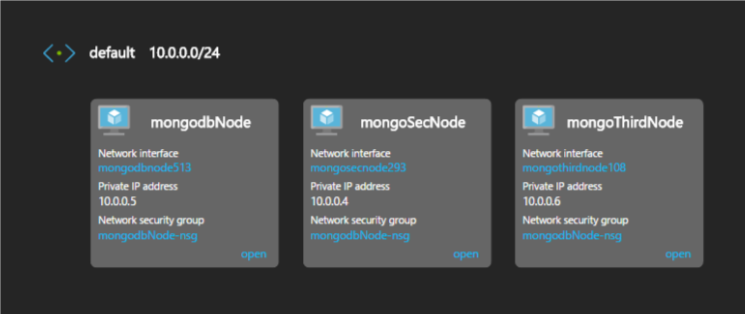
\includegraphics[scale=0.5]{privateNetwork}
	\caption{Sieć wirtualna}
\end{figure}

\subsubsection{Sieć publiczna}
Aby umożliwić połączenie z zestawem replik od dowolnego klienta, bez wymogu jego wdrożenia w chmurze \textit{Azure}, każdej z instancji maszyn wirtualnych został przydzielony publiczny adres IP, oraz nazwa DNS umożliwiająca dostęp do maszyn.

\subsection{Konfiguracja MongoDB}
Korzystając z \textit{mongo shell} utworzony został zestaw replik oraz jego konfiguracja. 

\begin{figure}[H]
	\centering
	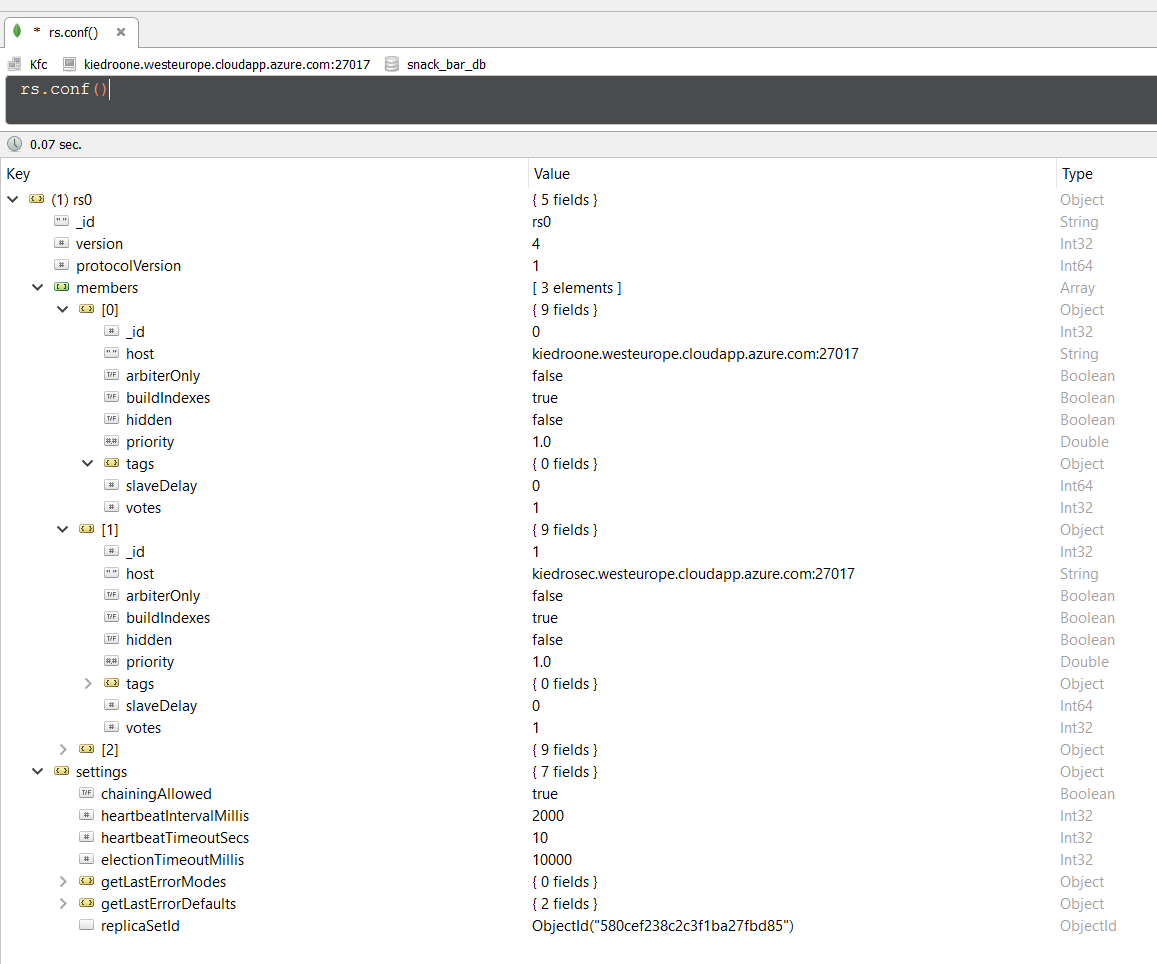
\includegraphics[width=\textwidth]{rsConfig}
	\caption{Konfiguracja zestawu replik}
\end{figure}

Korzystając z pliku konfiguracyjnego uaktywiono prosty interfejs REST, pozwalający na łatwą diagnozę zestawu replik.

\begin{figure}[H]
	\centering
	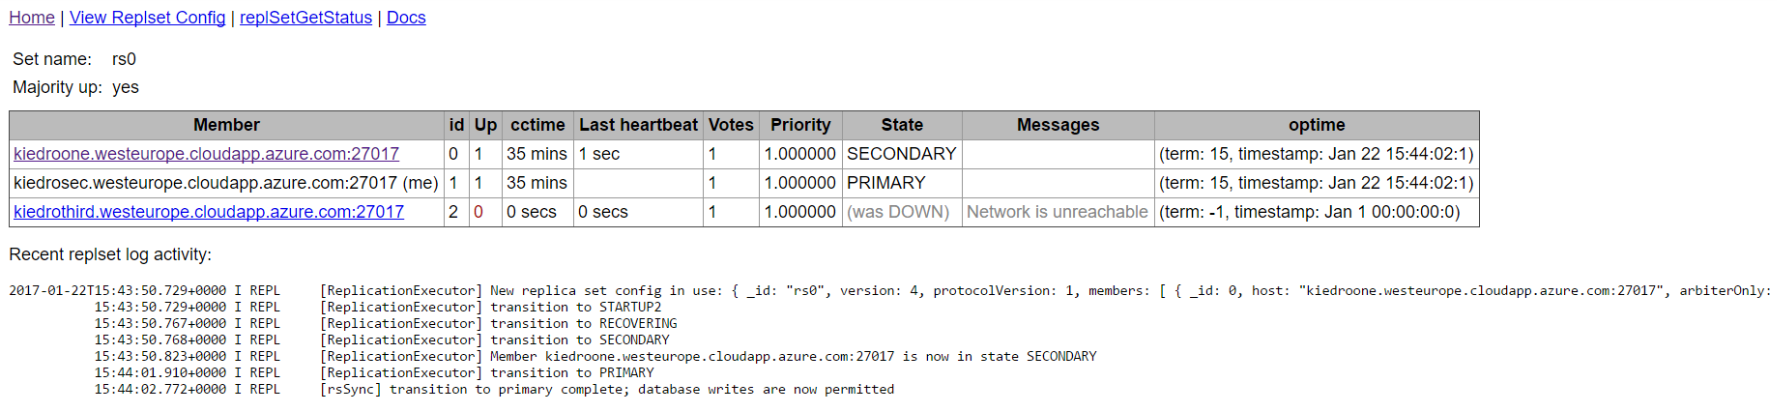
\includegraphics[width=\textwidth]{rest_interface}
	\caption{Interfejs REST}
\end{figure}

\subsection{Schemat bazy danych}
MongoDB należy do baz NoSQL typu dokumentowego, jedną z cech charaktrystycznych baz tego typu jest brak ustalonego schematu bazy danych. Kolekcje tworzone dynamicznie w trakcie działania aplikacji pozwalają na przechowywanie dowolnych danych - jedynym warunkiem jest możliwość ich serializacji w formacie JSON. \\
Ta cecha baz NoSQL upraszcza wstępną konfigurację bazy danych.

\subsection{Weryfikacja}
Do weryfikacji poprawnego działania bazy danych - możliwości połączenia ze wszystkimi węzłami, odczytu, zapisu, działania mechanizmu replikacji posłużyło narzędzie \textit{Robomongo} w wersji 0.9.

\begin{figure}[H]
	\centering
	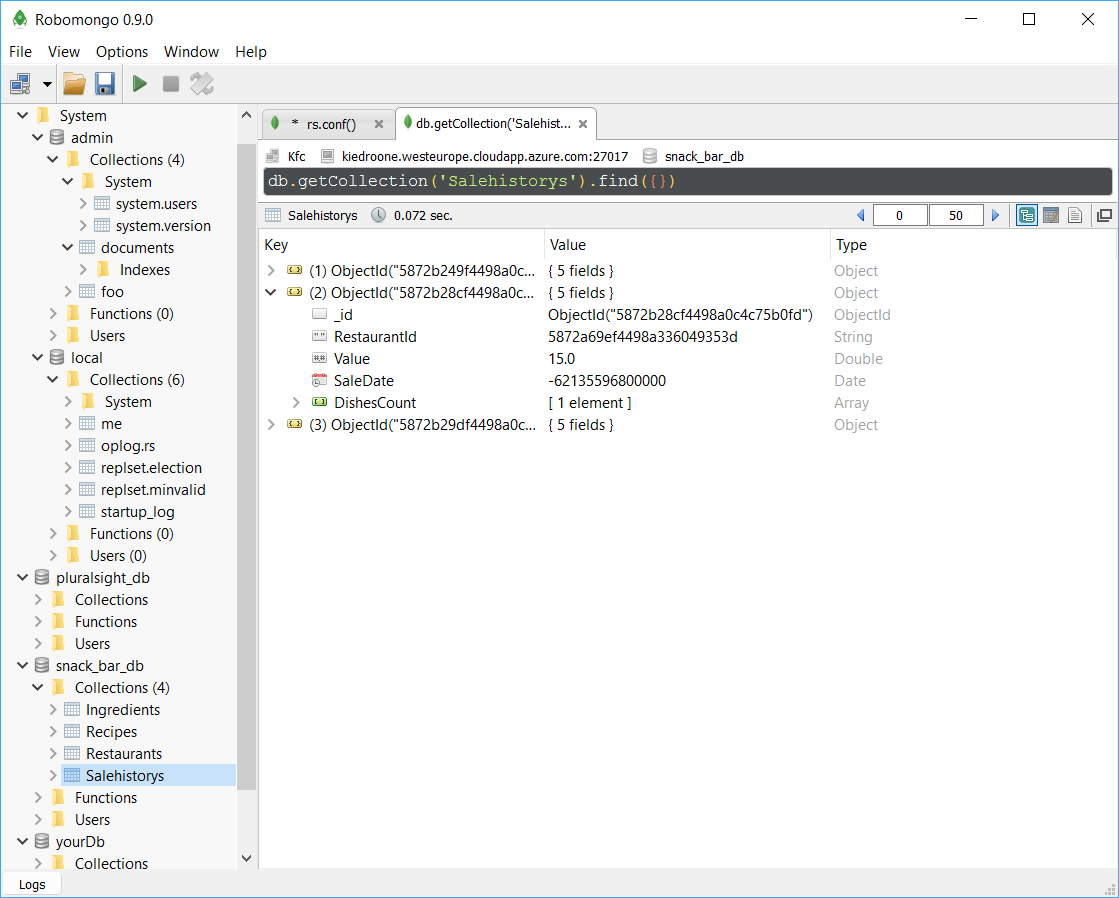
\includegraphics[width=\textwidth]{robomongo}
	\caption{Robomongo}
\end{figure}